\section{Verification, proposed source updates, and further research}
\label{sec:verification-research}

\subsection{Independent algebraic and numerical checks}

The arguments in this article are analytic proofs.  The accompanying
programs serve a separate purpose: they test constants, signs,
normalizations, branch choices, and the practical sizes of the
asymptotic errors.  They are neither interval certificates nor
formal proofs in a proof assistant.  The package records the programs,
their input grids, numerical precision, and complete outputs.

The finite-coefficient program computes the same quantities in three
ways.  For $s=3,u=4$, it compares the first eight coefficients from
\eqref{eq:lagrange-exact} with exact rational arithmetic in the original
implicit equation.  All eight agree exactly.  For a larger critical
case it compares the positive recurrence \eqref{eq:finite-E} at $n=64$
with an independent 75-digit evaluation; their relative difference
in the recorded environment is $1.22\cdot10^{-18}$.
It then computes the phase tests at $n=128,512,2048$ without
subtracting nearly equal coefficient contributions.

\begin{table}[htbp]
\centering
\caption{Computed coefficient divided by its leading equivalent
at $n=2048$.  These are finite-index diagnostics, not error bounds.}
\label{tab:phase-checks}
\begin{tabular}{@{}lll@{}}
\toprule
Regime & Parameters & Ratio\\
\midrule
Critical fractional & $s=2.5$, $u=\Uc(s)$ & $0.997778596$\\
Critical marginal & $s=3$, $u=\Uc(s)$ & $0.739119713$\\
Critical finite curvature & $s=4$, $u=\Uc(s)$ & $1.002010230$\\
Supercritical & $s=2.5$, $b=2A$ & $0.993099929$\\
Supercritical integer & $s=4$, $b=2A$ & $1.016617966$\\
Interior & $s=2.5$, $u=0.8\Uc(s)$ & $1.001610430$\\
Interior & $s=3$, $u=0.8\Uc(s)$ & $1.000008400$\\
Interior & $s=4$, $u=0.8\Uc(s)$ & $0.999995456$\\
\bottomrule
\end{tabular}
\end{table}

The marginal row is deliberately retained.  The leading order-three
law converges slowly because the effective expansion parameter is
$(\log\log n)/\log n$.  At $n=2048$ the coefficient is only
$73.9\%$ of its leading approximation.  In contrast, the coefficient
divided by the approximation through the second logarithmic correction
in \eqref{eq:three-term-log-law} is $1.010075657$.  The corresponding
ratios at $n=128$ and $512$ are $1.049782812$ and $1.020656682$.
This is useful evidence for the correction constants, while also
showing why the leading equivalent alone can be misleading at
computationally accessible indices.

\begin{figure}[htbp]
\centering
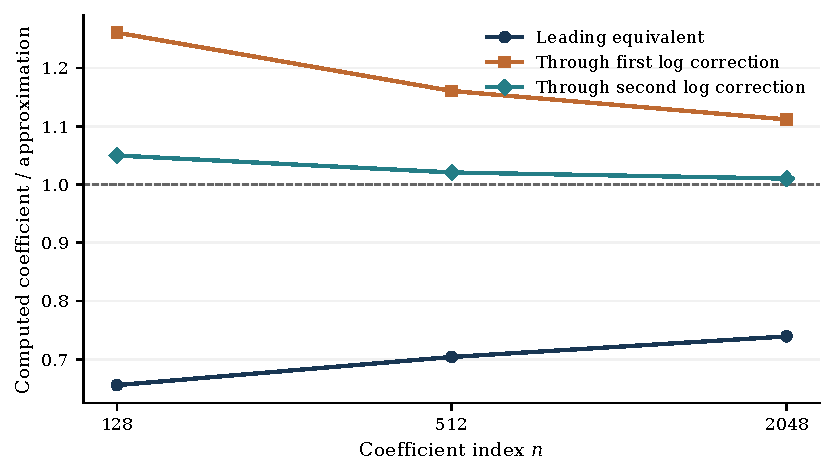
\includegraphics[width=0.83\textwidth]{figures/marginal_refinement.pdf}
\caption{The order-three coefficient divided by successive
asymptotic approximations.  Points are exact finite recurrences in
floating-point arithmetic; connecting segments only guide the eye.
The horizontal line is ratio one.  The three recorded indices are
$128$, $512$, and $2048$.}
\label{fig:marginal}
\end{figure}

For the inverse charts, a separate 180-digit program solves the
original polylogarithmic equation at $s=2.5,3,3.5,4$ and
$d=10^{-8},10^{-16},10^{-32}$.  The largest residual, divided by
$d$, is $1.89\cdot10^{-149}$ on this grid.  The same program verifies
the first core polynomials and the transferred logarithmic
corrections symbolically.  A 200-digit program independently checks
the critical order crossover for $\lambda=-2,0,2$ and $X=20,40,80$.
It evaluates both the original square-root deficit and the paired
equation.  At $X=80$, the observed relative errors after the second
algebraic correction range from $2.86\cdot10^{-6}$ to
$7.12\cdot10^{-5}$.  It also tests the exact first exponential
coefficient in \eqref{oc:first-exp-coefficient} against the difference
between the full solution and the complete algebraic core.
The separate joint-crossover program additionally tests nonzero
$\eta$, checks the selected real branch against the interior fold,
and includes a local complex-fold diagnostic; its complete parameters
and residuals are in \path{data/joint_crossover_checks.json}.
On the $18$-point joint grid, the maximum absolute relative error
of the first-corrected approximation decreases from $8.03\cdot10^{-3}$
at $X=40$ to $2.15\cdot10^{-3}$ at $X=80$.  All six negative-$\eta$
cases pass the independent fold-side check.  At the complex test
$k=1,X=40$, the full fold equations have tiny numerical residuals,
but the leading limiting constants still differ from the computed
$\alpha_c$ and $\omega_c$ by approximately $1.52$ and $0.317$,
respectively.  Solving the full equations accurately does not make
their leading asymptotic approximation equally accurate.

\begin{figure}[htbp]
\centering
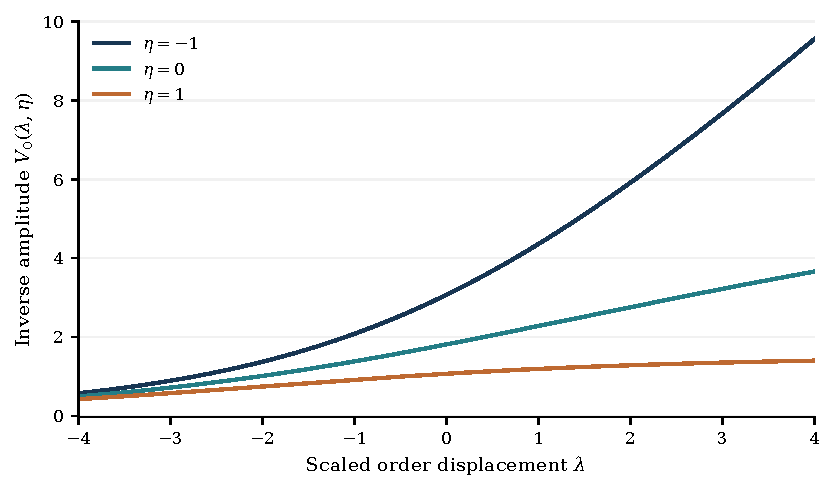
\includegraphics[width=0.87\textwidth]{figures/joint_profile.pdf}
\caption{The explicit positive profile $V_0(\lambda,\eta)$ in
\eqref{oc:profile}.  The curves are exact evaluations of the limiting
formula, not fitted numerical data.  They show how the order and
feedback displacements jointly determine the inverse amplitude.}
\label{fig:joint-profile}
\end{figure}

Finally, the coefficient-crossover program tests all $27$ combinations
of $s=2.5,3,4$, $n=128,512,2048$, and prescribed
$\xi=-1,0,1$.  The parameter $b$ is selected on the locally unique
branch near $A$, within $[A/2,2A]$.  This qualification matters:
for $s>3$ the map $b\mapsto\xi$ is not globally one-to-one on
$(0,\infty)$.  The stable density convention is independently checked
by 75-digit Fourier integration at $\xi=\pm1$ and by
\eqref{eq:stable-zero} at zero.  The largest relative difference from
the density evaluator is $5.15\cdot10^{-16}$.

\begin{figure}[htbp]
\centering
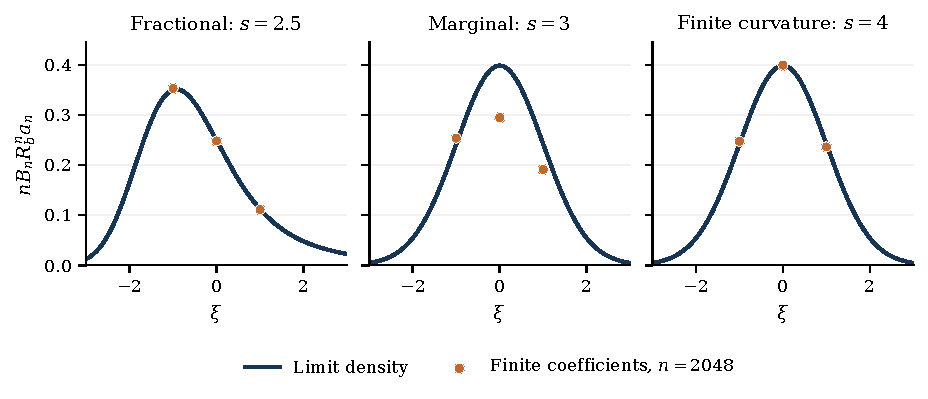
\includegraphics[width=\textwidth]{figures/coefficient_crossover.pdf}
\caption{Coefficient crossover in the normalization
$nB_n\Rb^n a_n$.  Curves are the stable or Gaussian limit densities;
points are the finite coefficient computation at $n=2048$ and
$\xi=-1,0,1$.  The elementary order-three normalization still has
visible logarithmic error.  Convergence need not be monotone at
every noncentral $\xi$.}
\label{fig:coefficient-crossover}
\end{figure}

\FloatBarrier
\subsection{What should change in the inspected material}

The source theorem for an interior characteristic point is correct in
its stated range.  Its boundary discussion was explicitly a proposed
research problem, so the missing proof should not be described as an
error.  The natural source update is to mark its supercritical
candidate as proved by \cref{thm:phase}, and replace its remaining
critical-endpoint question by the three exact laws
\eqref{eq:critical-stable}--\eqref{eq:critical-gaussian}.  The physical
convergence statement can then be extended from $0<s\le2$ to every
$s>0$ by \cref{cor:physical}.

The focused audit did not confirm a new false theorem in the inspected
incoming reports.  Several distinctions nevertheless need to survive
integration, because omitting them would create incorrect extensions:

\begin{enumerate}
\item \textbf{The endpoint reference is not always the Taylor radius.}
For $s>2$ and $b>0$, the equality $R=\Rb$ holds at and above the feedback threshold.
Below it, the physical germ first reaches an interior fold, whose
radius is larger than the endpoint reference.  The exact probability
identity still uses $\Rb$ on both sides.

\item \textbf{Integer orders require the paired expression.}
Gamma and zeta poles in the noninteger expansion cancel before any
integer limit.  For example the order-four term uses $H_3=11/6$,
not a separate value of $\zeta(1)$.  Similarly, the order-three
constant $5/2$ includes the quadratic feedback contribution.

\item \textbf{A function chart and a coefficient expansion have
different convergence claims.}
The charts in \cref{sec:charts,sec:order-crossover} are convergent
holomorphic substitutions.  The Gamma-derivative transfer series is
used only to a fixed asymptotic order.

\item \textbf{Local complex folds need a sheet qualification.}
\Cref{thm:local-complex-fold} describes continued local normal-form
solutions.  It does not locate a singularity of the original Taylor
germ without a separate global continuation argument.

\item \textbf{Uniformity requires stated parameter sets.}
In the lattice limit, $b$ stays in a compact positive interval.
The compact $\xi$ consequence then forces $b\to A$.  The theorem
does not cover an unrelated sequence $b\to0$, nor does an absolute
local-limit error prove a relative tail estimate in an expanding
$\xi$ window.
\end{enumerate}

The integration notes provide the source locations and a proposed
cross-reference paragraph.  They preserve the incoming source's
historical theorem labels and credit the earlier linear-tail models.
No existing theorem needs to be silently relabeled or removed.

\subsection{Further research questions and concrete targets}

The following questions are deliberately more specific than requests
for ``higher-order terms.''  Each identifies an additional statement
that is not proved by the present theorems.

\begin{enumerate}[label=\textbf{Q\arabic*.},leftmargin=2.7em]
\item \textbf{Joint coefficient asymptotics as both the order and
feedback vary.}
\Cref{thm:joint-crossover} treats the local inverse with varying
order; \cref{thm:coefficient-crossover} keeps the order fixed.
A natural next theorem would make the coefficient statement uniform
when
\[
 s_n=3+\eps_n,\qquad
 \lambda_n=\frac{\eps_n\log n}{2}
\]
stays bounded.  Pole pairing suggests the candidate scale
\[
 \widetilde B_n^2=\frac{n\log n}{2b_n}\ph(\lambda_n),
 \qquad
 \frac{n(1-\zeta(s_n-1)/b_n)}{\widetilde B_n}=O(1),
\]
and a Gaussian limit in this normalization.  This is a proposed
target, not a theorem claimed here.  The principal tasks are uniform
Fourier domination through the colliding poles, the first correction,
and comparison with the exact Lambert scale at $\lambda=0$.
The corresponding linear-tail results in \cite{RepoGaussian} are a
starting point, not a substitute for the nonlinear estimates.

\item \textbf{Relative matching in expanding crossover windows.}
Determine the largest positive and negative ranges of $\xi_n$ in
which a relative version of \eqref{eq:crossover-coefficient} holds.
On the positive side it should match the fixed supercritical
$n^{-s}$ law; on the negative side it should match the interior-fold
exponential factor.  Such a result requires a uniform large-deviation
or saddle analysis beyond the absolute local limit.

\item \textbf{Quantitative convergence radii for the charts.}
The holomorphic implicit function theorem supplies positive radii
uniformly on compact parameter sets, but not optimal computable ones.
Find certified polydiscs for the low-order, Lambert, and joint charts,
and rigorous truncation constants that can be used numerically.
The coefficient functions' possible pole at $w=2$ is an algebraic
clue; it is not already a determination of the chart's global boundary.

\item \textbf{Global access to the complex fold curves.}
For fixed nonzero $k$, decide which paths in the complex order and
feedback variables carry the original germ to the local branches of
\cref{thm:local-complex-fold}.  Determine their monodromy and whether
they ever become dominant singularities of a specified continuation.
The local two-sheet normal form alone cannot answer this question.

\item \textbf{All coefficient corrections away from the marginal
order.}
Transfer the exact charts into finite formulas for every correction
in the stable range and at higher orders, including cancellations
when different chart monomials produce the same power.  At rational
orders, distinguish merging exponents from zeros of reciprocal Gamma
factors.  The conditional disappearance of the ladder at
$\zeta(s-2)=-1$ gives a particularly clean test case.

\item \textbf{General analytic feedback potentials.}
Replace $uv-v^2/2$ by an analytic $F(v)$ with $F(0)=0$ and study
$F(v)=\Li_s(r\ee^v)$.  For $s>3$, if $F(v_b)=\zeta(s)$ and
$F'(v_b)=\zeta(s-1)$, the finite-curvature term is governed by
$\zeta(s-2)-F''(v_b)$.  Find hypotheses preserving positive
coefficients and global dominance, and classify what happens when
this curvature is tuned to zero.  The latter can create a higher
degeneracy and needs a different chart.

\item \textbf{Logarithmically weighted and slowly varying tails.}
Replace $k^{-s}$ by $k^{-s}(\log k)^q$, or by
$k^{-s}L(k)$ under explicit regularity assumptions.  Order derivatives
of the polylogarithm give exact finite logarithmic weights, linking
this problem to the incoming order-jet articles.  Determine which
tails still admit convergent finite-generator charts and which yield
only asymptotic scales.  A regular-variation equivalent alone cannot
imply an analytic convergent chart.

\item \textbf{Arithmetic support and several dominant points.}
The uniqueness proof uses the positivity of every coefficient.
For feedback supported on a proper lattice, classify the competing
root-of-unity singularities and the resulting periodic coefficient
laws.  More generally, identify the least support hypotheses under
which the strict triangle argument and aperiodic local limit remain
valid.

\item \textbf{Finite action cutoffs in the nonlinear kernel.}
Study truncations before and after the nonlinear transformation
$f_u(t)=u-\sqrt{u^2-2\Li_s(t)}$.  These are different operations.
Determine the cutoff required to preserve each critical coefficient
law and the crossover profile, and whether the prefix cancellations
in the linear endpoint literature survive the quadratic feedback.

\item \textbf{Certified and formal verification.}
Convert the finite coefficient recursions and Lagrange extraction
identities into proof-assistant statements first.  An interval
implementation of the sector bounds and Rouch\'e circles could then
certify explicit numerical domains.  Formalizing the global
continuation and logarithmic transfer steps is a separate, larger
project; the supplied numerical scripts do not accomplish it.
\end{enumerate}

Questions Q1--Q3 offer the most direct continuation of the present
analysis.  Q4 and Q6 address genuinely additional analytic structure;
Q7--Q9 connect the exact model to broader tail classes and the action
budgets already studied in the repository.  The existing finite
identities, positivity argument, and pole-paired normal form provide
concrete starting points for each direction.

\subsection{Reproducibility and integration}

The archive contains the master \path{article.tex}, its seven section
files, the bibliography source, the compiled PDF, five verification
programs, a figure-generation program, machine-readable records,
and integration notes.  The recorded data permit the figures and PDF
to be rebuilt without rerunning high-precision roots.  The optional
verification target recomputes all numerical and symbolic checks.
The README gives the commands, dependency versions, and a distinction
between exact arithmetic checks and numerical diagnostics.
The source provenance pins the repository revision and hashes the
specific comparison files and incoming archives.
